\chapter{أين تعيش الحيوانات}\label{ch:g2:where-animals-live}

لن تلقى سمكة سلمون مرقط في ساحة المدرسة، ولا سنجابًا في قاع
البركة. فكل \omterm{def:g1:animals-around-us:animal}{حيوان} يعيش في المكان الذي يناسبه --- حيث يجد غذاءه
ومأواه وجيرانه. ولعلماء الأحياء اسم لأرض \omterm{def:g1:animals-around-us:animal}{الحيوان} التي يقيم فيها.

\section{الموائل}

\begin{definition}[الموئل]\label{def:g2:where-animals-live:habitat}
\emph{موئل}\index{موئل} \omterm{def:g1:animals-around-us:animal}{الحيوان} هو نوع المكان الذي يعيش فيه على
نحو طبيعي ويجد فيه كل ما يحتاج إليه: الغذاء، والماء، والمأوى،
وموضعًا آمنًا لصغاره. فالبركة، والغابة، والمرج، والسياج النباتي،
وشاطئ البحر موائل.
\end{definition}

\begin{example}[أربعة موائل وأربعة أحياء]\label{ex:g2:where-animals-live:four}
في \emph{البركة}: ضفادع، ورعاشات، وأسماك شوكية، وحلزونات ماء. وفي
\emph{الغابة}: سناجب، وأيائل، ونقّارات خشب، ونمل الخشب. وفي
\emph{المرج}: أرانب، وجنادب، وفراشات، وفئران حقل. وتحت حجارة
\emph{جدار} قديم: حشرات القمل الخشبي، وعناكب، وأحيانًا سحلية
تتشمس فوقه.
\end{example}

\begin{omfigure}
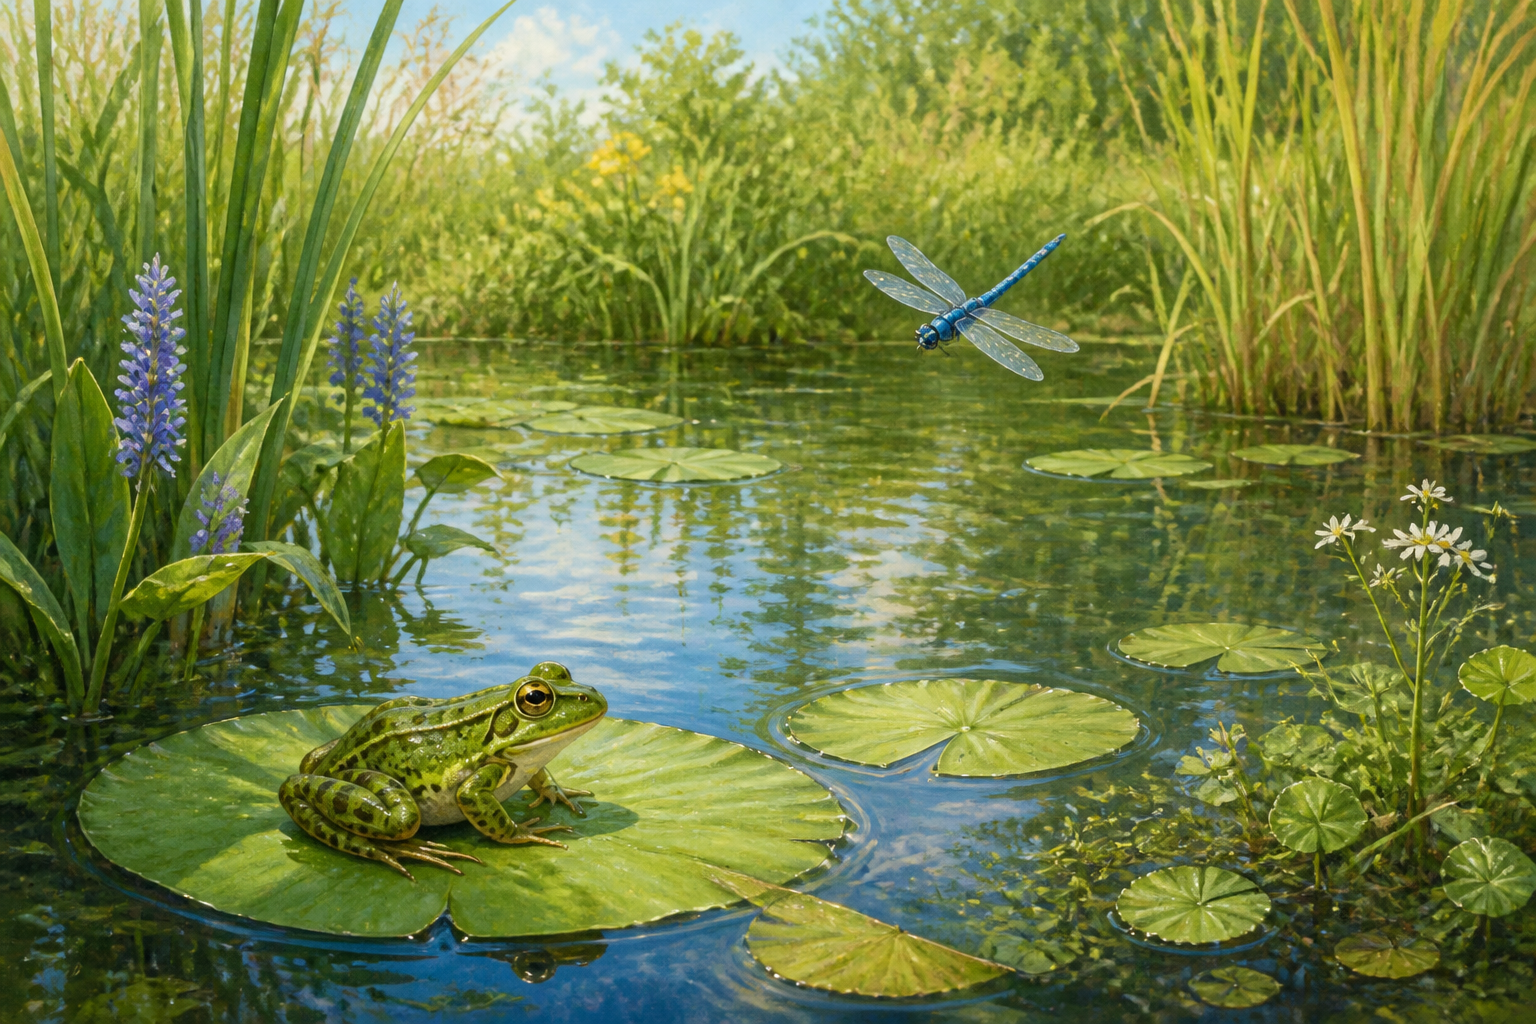
\includegraphics[width=0.62\linewidth]{images/book1/ai/g2-live-pond.png}

{\small \omterm{def:g2:where-animals-live:habitat}{موئل} البركة واثنان من سكانه في بيتهما: ضفدع على \omterm{def:g1:plants-around-us:parts}{ورقة} نيلوفر،
ورعّاشة في دورية.}
\end{omfigure}

\begin{omfigure}
\begin{tikzpicture}[scale=0.88]
  \draw[thick, omDef, fill=omDef!7, rounded corners=6pt]
    (0,0) rectangle (3.4,2.6);
  \draw[thick, omMeth, fill=omMeth!7, rounded corners=6pt]
    (3.9,0) rectangle (7.3,2.6);
  \draw[thick, omProp, fill=omProp!7, rounded corners=6pt]
    (7.8,0) rectangle (11.2,2.6);
  \node[font=\small\bfseries, omDef] at (1.7,2.25) {البركة};
  \node[font=\small\bfseries, omMeth] at (5.6,2.25) {الغابة};
  \node[font=\small\bfseries, omProp] at (9.5,2.25) {المرج};
  \node[font=\small, align=center] at (1.7,1.05)
    {ضفدع\\ رعّاشة\\ سمكة شوكية};
  \node[font=\small, align=center] at (5.6,1.05)
    {سنجاب\\ نقّار خشب\\ أيّل};
  \node[font=\small, align=center] at (9.5,1.05)
    {أرنب\\ جندب\\ فراشة};
\end{tikzpicture}

{\small ثلاثة \omterm{def:g2:where-animals-live:habitat}{موائل} وبعض سكانها. جرّب أن تبدّل بينها --- فالسنجاب
لن يدوم طويلًا في البركة.}
\end{omfigure}

\begin{remark}[موئل واحد وبيوت كثيرة]\label{rem:g2:where-animals-live:layers}
\omterm{def:g2:where-animals-live:habitat}{للموئل} زوايا كثيرة. ففي الغابة الواحدة يعيش نقّار الخشب عاليًا على
الجذوع، والسنجاب في \omterm{def:g1:plants-around-us:tree}{الأغصان}، والأيّل بين الشجيرات، ونمل الخشب على
الأرض في عشه المكوّم. الغابة نفسها، وطوابق مختلفة --- ولذلك تستطيع
\omterm{def:g1:animals-around-us:animal}{حيوانات} كثيرة أن تتشارك موئلًا واحدًا من غير ازدحام.
\end{remark}

\section{مهيَّأ لموئله}

\begin{proposition}[الحيوانات تناسب موائلها]\label{prop:g2:where-animals-live:fit}
جسم \omterm{def:g1:animals-around-us:animal}{الحيوان} وعاداته يناسبان المكان الذي يعيش فيه:
\begin{itemize}
  \item قدما الضفدع المكفوفتان تدفعان الماء --- فهما مصنوعتان
        للبركة؛
  \item ومخالب السنجاب القابضة وذنبه الكبير الموازن مصنوعان
        للأشجار؛
  \item وكفّا الأرنب الحافرتان وأذناه الطويلتان المنذرتان مصنوعة
        لمرج مفتوح تحته جحور؛
  \item \omterm{def:g1:animals-around-us:covering}{وريش} البطة يدفع الماء، وقدماها المكفوفتان تجدّفان.
\end{itemize}
وإذا نُقل \omterm{def:g1:animals-around-us:animal}{الحيوان} إلى \omterm{def:g2:where-animals-live:habitat}{الموئل} الخطأ فقد هذه المزايا.
\end{proposition}
\admitted

\begin{example}[عتاد الخُلد]\label{ex:g2:where-animals-live:mole}
يعيش الخُلد تحت الأرض، في أنفاق يحفرها تحت المرج. ويداه مجرفتان
عريضتان للحفر، وفروه ينبطح في الاتجاهين معًا فلا تشعّثه التربة،
وعيناه الضعيفتان لا تكادان تهمّان في الظلام. وهو فوق الأرض أخرق؛
أما في موئله فبطل.
\end{example}

\begin{method}[مقارنة حيوان بموئله]\label{met:g2:where-animals-live:matching}
إذا أُعطيت حيوانًا غير مألوف:
\begin{enumerate}
  \item انظر إلى عتاده: أقدم مكفوفة؟ أم مخالب؟ أم أجنحة؟ أم كفّا
        حفر؟
  \item واسأل ماذا يأكل، وأين يوجد ذلك الغذاء؛
  \item واسأل أين يستطيع أن يأوي ويربّي صغاره؛
  \item \omterm{def:g2:where-animals-live:habitat}{والموئل} الذي يجيب عن الثلاثة جميعًا هو بيته المرجح.
\end{enumerate}
\end{method}

\section{الموائل يمكن أن تُفقد}

\begin{proposition}[لا موئل، فلا سكان]\label{prop:g2:where-animals-live:loss}
لا يستطيع \omterm{def:g1:animals-around-us:animal}{الحيوان} أن يعيش بلا موئله. فإذا رُدمت بركة اختفت معها
ضفادعها ورعّاشاتها؛ وإذا اقتُلع سياج نباتي فقدت الطيور التي عشّشت
فيه مأواها. وحماية \omterm{def:g1:animals-around-us:animal}{الحيوانات} تبدأ بحماية الأماكن التي تعيش فيها.
\end{proposition}
\admitted

\begin{example}[بركة المدرسة]\label{ex:g2:where-animals-live:schoolpond}
تحفر مدرسة بركة صغيرة في ركن من ساحتها. وفي غضون سنتين تجوب
الرعّاشات فوقها، ويمشي عليها بعوض الماء، وتنتقل الضفادع إليها ---
ولم يجلبها أحد. اصنع \omterm{def:g2:where-animals-live:habitat}{الموئل}، فيجده السكان.
\end{example}

\begin{remark}[النظر من غير إزعاج]\label{rem:g2:where-animals-live:respect}
حين نزور موئلًا فنحن ضيوف. فانظر في هدوء، وأعد الحجارة كما وجدتها،
ودع \omterm{def:g2:animals-grow-up:born}{البيض} والأعشاش وشأنها، واحمل نفاياتك معك إلى البيت --- ينبغي
أن ينسى \omterm{def:g2:where-animals-live:habitat}{الموئل} أنك كنت هناك. والفصول التالية تعطي طرقًا أخرى
للعناية بالطبيعة.
\end{remark}

\section{تمارين}

\begin{exercise}[$\star$]\label{exo:g2:where-animals-live:1}
ما \omterm{def:g2:where-animals-live:habitat}{الموئل}؟ وسمِّ الأشياء الأربعة التي يجدها \omterm{def:g1:animals-around-us:animal}{الحيوان} فيه.
\end{exercise}

\begin{exercise}[$\star$]\label{exo:g2:where-animals-live:2}
اذكر حيوانين من البركة، واثنين من الغابة، واثنين من المرج.
\end{exercise}

\begin{exercise}[$\star$]\label{exo:g2:where-animals-live:3}
أي \omterm{def:g2:where-animals-live:habitat}{موئل} يناسب كل \omterm{def:g1:animals-around-us:animal}{حيوان}: السمكة الشوكية، ونقّار الخشب، والجندب،
وحشرة القمل الخشبي؟
\end{exercise}

\begin{exercise}[$\star$]\label{exo:g2:where-animals-live:4}
ما عتاد السباحة عند الضفدع؟ وما عتاد تسلق الأشجار عند السنجاب؟
\end{exercise}

\begin{exercise}[$\star$]\label{exo:g2:where-animals-live:5}
عدّد قطع عتاد الخُلد الثلاث تحت الأرض من
\cref{ex:g2:where-animals-live:mole}.
\end{exercise}

\begin{exercise}[$\star$]\label{exo:g2:where-animals-live:6}
في \cref{rem:g2:where-animals-live:layers}، أي ``طابق'' من الغابة
يستعمله كل \omterm{def:g1:animals-around-us:animal}{حيوان}: نقّار الخشب، والسنجاب، والأيّل، ونملة الخشب؟
\end{exercise}

\begin{exercise}[$\star$]\label{exo:g2:where-animals-live:7}
ماذا يحدث للضفادع والرعّاشات حين تُردم بركة؟ وماذا يعلّمنا ذلك عن
حماية \omterm{def:g1:animals-around-us:animal}{الحيوانات}؟
\end{exercise}

\begin{exercise}[$\star$]\label{exo:g2:where-animals-live:8}
جرّب: اختر موئلًا صغيرًا قريبًا منك --- تحت حجر، أو شجيرة، أو حوض
زهور. راقب في هدوء وعدّد كل \omterm{def:g1:animals-around-us:animal}{حيوان} تراه في مدة محددة. وأعد كل حجر
إلى مكانه. كم ساكنًا كان في موئلك الصغير؟
\end{exercise}

\begin{exercise}[$\star\star$]\label{exo:g2:where-animals-live:9}
\omterm{def:g1:animals-around-us:animal}{حيوان} غامض له قدمان مكفوفتان، \omterm{def:g1:animals-around-us:covering}{وريش} كثيف يدفع الماء، ومنقار مسطح
للغربلة. استعمل \cref{met:g2:where-animals-live:matching} لتسمية
موئله --- ولعلك تسمي \omterm{def:g1:animals-around-us:animal}{الحيوان} نفسه.
\end{exercise}

\begin{exercise}[$\star\star$]\label{exo:g2:where-animals-live:10}
يريد توم أن ``يساعد'' ضفدعًا بأخذه إلى بيته في حوض جاف مع طعام
وفير. استعمل \cref{prop:g2:where-animals-live:fit}
و\cref{prop:g2:where-animals-live:loss} لتشرح لماذا لا يفيد هذا
الضفدع البتة.
\end{exercise}
